\documentclass[11pt, a4paper]{article}

% ── Packages ──────────────────────────────────────────────────────────────
\usepackage[margin=1in]{geometry}
\usepackage{graphicx}
\usepackage{booktabs}
\usepackage{longtable}
\usepackage{enumitem}
\usepackage{xcolor}
\usepackage{hyperref}
\usepackage{listings}
\usepackage{tikz}
\usetikzlibrary{shapes.geometric, arrows.meta, positioning, fit, calc}
\usepackage{amsmath}
\usepackage{caption}
\usepackage{float}

% ── Colors ────────────────────────────────────────────────────────────────
\definecolor{newcode}{RGB}{0, 100, 0}       % dark green — new RH code
\definecolor{reused}{RGB}{0, 70, 140}       % dark blue  — reused from OptiChat
\definecolor{shared}{RGB}{140, 80, 0}       % dark orange — shared infra
\definecolor{codebg}{RGB}{245, 245, 245}
\definecolor{codeframe}{RGB}{200, 200, 200}

\hypersetup{
    colorlinks=true,
    linkcolor=black,
    urlcolor=reused,
    citecolor=black,
}

\lstset{
    basicstyle=\ttfamily\small,
    backgroundcolor=\color{codebg},
    frame=single,
    rulecolor=\color{codeframe},
    breaklines=true,
    columns=fullflexible,
    keepspaces=true,
    showstringspaces=false,
}

% ── Title ─────────────────────────────────────────────────────────────────
\title{%
    \textbf{Rolling Horizon Comparison Framework} \\[6pt]
    \large A Wrapper Module over OptiChat for Multi-Period \\
    Optimization Model Comparison
}
\author{Shreyas Kompalli}
\date{\today}

% ══════════════════════════════════════════════════════════════════════════
\begin{document}
\maketitle

\begin{abstract}
This document describes the \textbf{Rolling Horizon (RH) Comparison Framework},
a self-contained module built on top of the existing \textsc{OptiChat} system.
The framework enables users to compare two versions of an optimization model
across time periods or scenarios, answering questions such as \emph{``What
changed?''}, \emph{``Would the old plan still work?''}, and \emph{``What drove
the changes?''}.  The document clearly identifies which components are
\textcolor{newcode}{\textbf{newly created}} for the RH framework, which are
\textcolor{reused}{\textbf{reused}} from the existing OptiChat codebase, and
which represent \textcolor{shared}{\textbf{shared infrastructure}}.
\end{abstract}

\tableofcontents
\newpage

% ══════════════════════════════════════════════════════════════════════════
\section{Overview}
% ══════════════════════════════════════════════════════════════════════════

OptiChat is a multi-agent conversational system that helps users interact with
optimization models through natural language.  The Rolling Horizon Comparison
Framework extends OptiChat by adding the ability to \emph{compare} two solved
model instances (called \textbf{Epoch~A} and \textbf{Epoch~B}) and explain the
differences to a non-technical user.

\subsection{Design Principle}

The RH framework is implemented as a \textbf{separate, self-contained module}
(\texttt{rh\_comparison/}) that lives alongside OptiChat but does \emph{not}
modify any existing OptiChat code.  The only integration points are:

\begin{enumerate}[leftmargin=2em]
    \item \textbf{LLM model imports} --- the RH agents reuse OptiChat's
          pre-configured LLM model handles (\texttt{gpt\_5\_mini} and
          \texttt{gpt\_5}) so that both systems share the same API keys and
          model configuration.
    \item \textbf{ADK API server} --- both apps are registered on the same
          Google ADK server (port 8000), sharing the session protocol.
    \item \textbf{Streamlit UI} --- \texttt{app.py} hosts both modes behind a
          radio-button selector.
\end{enumerate}

Everything else --- state management, data persistence, analytics, prompt
engineering, and tool definitions --- is newly written for the RH framework.

\subsection{Legend}

Throughout this document, the following colour coding is used:

\begin{itemize}[leftmargin=2em]
    \item \textcolor{newcode}{\textbf{Green}} --- Newly created for the RH framework
    \item \textcolor{reused}{\textbf{Blue}} --- Reused from the existing OptiChat codebase
    \item \textcolor{shared}{\textbf{Orange}} --- Shared infrastructure (not from OptiChat, but used by both)
\end{itemize}


% ══════════════════════════════════════════════════════════════════════════
\section{Architecture}
% ══════════════════════════════════════════════════════════════════════════

\subsection{High-Level Architecture Diagram}

\begin{figure}[H]
\centering
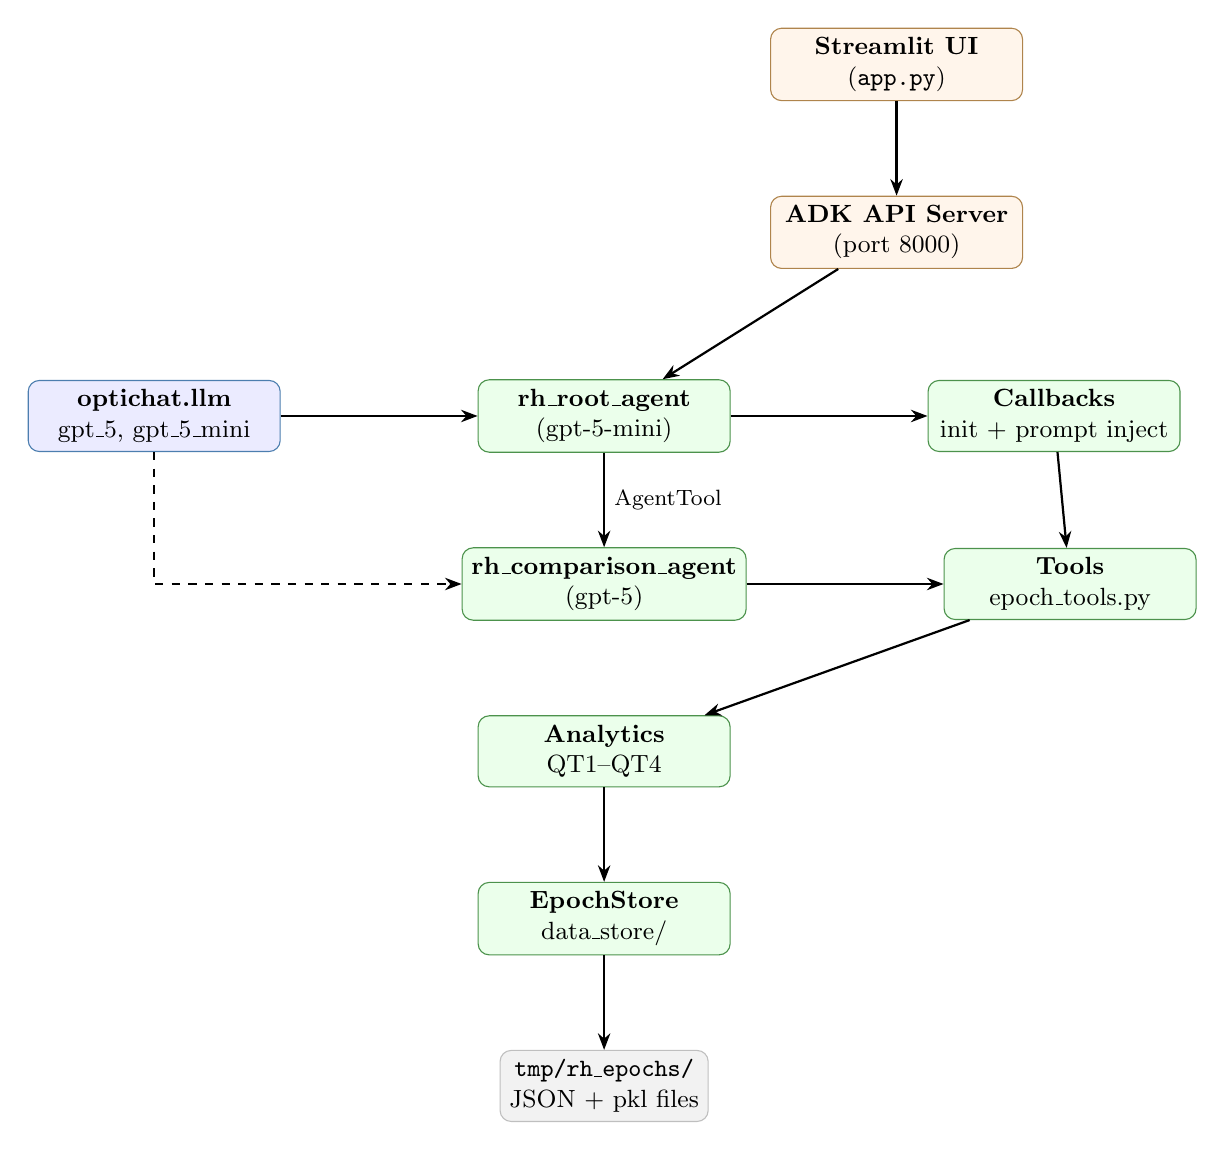
\begin{tikzpicture}[
    node distance=1.2cm and 2cm,
    every node/.style={font=\small},
    block/.style={rectangle, draw, rounded corners, minimum width=3.2cm, minimum height=0.9cm, align=center},
    newblock/.style={block, fill=green!8, draw=newcode!70},
    reusedblock/.style={block, fill=blue!8, draw=reused!70},
    sharedblock/.style={block, fill=orange!8, draw=shared!70},
    datablock/.style={block, fill=gray!10, draw=gray!50, minimum width=2.6cm},
    arr/.style={-{Stealth[length=6pt]}, thick},
]

% ── User layer ──
\node[sharedblock] (ui) {\textbf{Streamlit UI}\\(\texttt{app.py})};

% ── Server layer ──
\node[sharedblock, below=of ui] (server) {\textbf{ADK API Server}\\(port 8000)};

% ── Agent layer ──
\node[newblock, below left=1.4cm and 0.5cm of server] (root) {\textbf{rh\_root\_agent}\\(gpt-5-mini)};
\node[newblock, below=of root] (comp) {\textbf{rh\_comparison\_agent}\\(gpt-5)};

% ── Callbacks ──
\node[newblock, right=2.5cm of root] (callbacks) {\textbf{Callbacks}\\init + prompt inject};

% ── Tools ──
\node[newblock, right=2.5cm of comp] (tools) {\textbf{Tools}\\epoch\_tools.py};

% ── Analytics ──
\node[newblock, below=of comp] (analytics) {\textbf{Analytics}\\QT1--QT4};

% ── Data layer ──
\node[newblock, below=of analytics] (store) {\textbf{EpochStore}\\data\_store/};

% ── LLM import ──
\node[reusedblock, left=2.5cm of root] (llm) {\textbf{optichat.llm}\\gpt\_5, gpt\_5\_mini};

% ── Disk ──
\node[datablock, below=of store] (disk) {\texttt{tmp/rh\_epochs/}\\JSON + pkl files};

% ── Arrows ──
\draw[arr] (ui) -- (server);
\draw[arr] (server) -- (root);
\draw[arr] (root) -- node[right, font=\footnotesize]{AgentTool} (comp);
\draw[arr] (root.east) -- ++(0.5, 0) |- (callbacks.west);
\draw[arr] (comp.east) -- ++(0.5, 0) |- (tools.west);
\draw[arr] (callbacks) -- (tools);
\draw[arr] (tools) -- (analytics);
\draw[arr] (analytics) -- (store);
\draw[arr] (store) -- (disk);
\draw[arr] (llm) -- (root);
\draw[arr, dashed] (llm) |- (comp);

\end{tikzpicture}
\caption{High-level architecture of the Rolling Horizon Comparison Framework.
Green = new RH code; blue = reused from OptiChat; orange = shared infrastructure.}
\label{fig:architecture}
\end{figure}


\subsection{Directory Structure}

\begin{lstlisting}
rh_comparison/
|-- __init__.py                   # Entry point (re-export)
|-- rh_agent.py                   # Delegates to agents/rh_root_agent.py
|-- config/
|   +-- rh_constants.py           # State keys, thresholds, QueryType enum
|-- agents/
|   |-- rh_root_agent.py          # Root agent factory (classify + route)
|   |-- rh_comparison_agent.py    # Expert agent factory (answer questions)
|   +-- rh_prompts.py             # All prompt templates + QT formatters
|-- tools/
|   |-- rh_callback_tool.py       # ADK callbacks (init + prompt injection)
|   +-- epoch_tools.py            # ADK tool definitions + token-budget caps
|-- data_store/
|   +-- epoch_store.py            # EpochStore class + Pyomo model loader
+-- analytics/
    |-- __init__.py               # Re-exports compute_* functions
    |-- structural_diff.py        # QT1 — structural & parametric diff
    |-- solution_diff.py          # QT2 — solution value diff
    |-- backward_compat.py        # QT3 — backward compatibility check
    +-- attribution_analysis.py   # QT4 — solution attribution
\end{lstlisting}

All files above are \textcolor{newcode}{\textbf{newly created}}.
The only imports from OptiChat are \texttt{gpt\_5} and \texttt{gpt\_5\_mini}
from \texttt{optichat.llm}.


% ══════════════════════════════════════════════════════════════════════════
\section{Data Flow: From Upload to Answer}
% ══════════════════════════════════════════════════════════════════════════

The end-to-end data flow proceeds in two phases:

\subsection{Phase 1: Session Initialization}

When the user uploads two model files and clicks \emph{Initialize}, the
following happens:

\begin{enumerate}[leftmargin=2em]
    \item \textcolor{shared}{\texttt{app.py}} saves uploaded files to
          \texttt{tmp/rh\_uploads/} and builds an RH JSON config containing
          file paths, labels, and upload mode.
    \item The config is sent as a user message to the
          \textcolor{shared}{ADK API server}.
    \item The \textcolor{newcode}{\texttt{rh\_initialize\_session}} callback
          (registered as \texttt{before\_agent\_callback} on the root agent)
          intercepts the first message:
    \begin{enumerate}
        \item Loads each Pyomo model from the \texttt{.py} file
              (optionally injecting data from a \texttt{.json} file).
        \item Solves each model using Gurobi.
        \item Creates an \textcolor{newcode}{\texttt{EpochStore}} for each
              epoch, extracting and persisting
              \texttt{solution.json}, \texttt{params.json},
              \texttt{structure.json}, and \texttt{model.pkl}.
        \item Computes \textbf{QT1} (structural diff) eagerly.
        \item Generates natural-language model descriptions.
        \item Returns a structured initialization summary directly
              (no LLM call needed).
    \end{enumerate}
\end{enumerate}

\subsection{Phase 2: Question Answering}

When the user asks a question (e.g., ``Did any parameter values change?''):

\begin{enumerate}[leftmargin=2em]
    \item The \textcolor{shared}{ADK server} routes the message to
          \textcolor{newcode}{\texttt{rh\_root\_agent}}.
    \item The \textcolor{newcode}{\texttt{rh\_check\_llm\_request}} callback
          rebuilds the root agent's system prompt with current session metadata.
    \item The root agent's LLM (\textcolor{reused}{gpt-5-mini}) classifies
          the question into one of six query types and calls
          \textcolor{newcode}{\texttt{set\_query\_type()}} to register the
          classification in session state.
    \item The root agent delegates to
          \textcolor{newcode}{\texttt{rh\_comparison\_agent}} via
          \texttt{AgentTool}.
    \item The \textcolor{newcode}{\texttt{rh\_check\_llm\_request}} callback
          fires again for the comparison agent:
    \begin{enumerate}
        \item Reads the query type from session state.
        \item Computes any missing QT results on demand (e.g., QT3
              requires 1 Gurobi solver call).
        \item Assembles the full system prompt: base rules + epoch metadata
              + epoch descriptions + the relevant QT data block (formatted
              by \texttt{\_format\_qt\{1--4\}}) + strategy section.
    \end{enumerate}
    \item The comparison agent's LLM (\textcolor{reused}{gpt-5}) generates
          a natural-language answer, optionally calling
          \textcolor{newcode}{\texttt{get\_epoch\_data()}} or
          \textcolor{newcode}{\texttt{get\_comparison\_json()}} for
          drill-down data.
    \item The answer flows back through the root agent to the
          \textcolor{shared}{Streamlit UI}.
\end{enumerate}


% ══════════════════════════════════════════════════════════════════════════
\section{Newly Created Components}
\label{sec:new}
% ══════════════════════════════════════════════════════════════════════════

This section documents every function and class created specifically for the
RH framework, grouped by module.

% ─────────────────────────────────────────────────
\subsection{Agent Factories}
% ─────────────────────────────────────────────────

\subsubsection{\texttt{rh\_root\_agent.py}}

\begin{longtable}{p{5.5cm} p{9cm}}
\toprule
\textbf{Function} & \textbf{Description} \\
\midrule
\texttt{create\_rh\_root\_agent()} &
    Factory that creates the root ADK \texttt{Agent} for query
    classification and routing.  Registers two callbacks
    (\texttt{rh\_initialize\_session}, \texttt{rh\_check\_llm\_request})
    and two tools (\texttt{set\_query\_type}, \texttt{AgentTool} wrapping
    the comparison agent).  Uses \textcolor{reused}{\texttt{gpt\_5\_mini}}
    as the underlying LLM. \\
\bottomrule
\end{longtable}

\subsubsection{\texttt{rh\_comparison\_agent.py}}

\begin{longtable}{p{5.5cm} p{9cm}}
\toprule
\textbf{Function} & \textbf{Description} \\
\midrule
\texttt{create\_rh\_comparison\_agent()} &
    Factory that creates the expert ADK \texttt{Agent} for answering user
    questions.  Registers one callback (\texttt{rh\_check\_llm\_request})
    and two tools (\texttt{get\_epoch\_data}, \texttt{get\_comparison\_json}).
    Uses \textcolor{reused}{\texttt{gpt\_5}} as the underlying LLM. \\
\bottomrule
\end{longtable}


% ─────────────────────────────────────────────────
\subsection{Prompt Engineering (\texttt{rh\_prompts.py})}
% ─────────────────────────────────────────────────

\subsubsection{Prompt Constants}

\begin{longtable}{p{5.5cm} p{9cm}}
\toprule
\textbf{Constant} & \textbf{Purpose} \\
\midrule
\texttt{ROOT\_AGENT\_PROMPT\_TEMPLATE} &
    System prompt template for the root agent.  Contains session status,
    epoch metadata, query type definitions, and the 4-step workflow
    (classify $\to$ set type $\to$ delegate $\to$ return verbatim). \\
\midrule
\texttt{COMPARISON\_BASE\_PROMPT} &
    System prompt for the comparison agent.  Contains 5 rules:
    (1)~no code names, (2)~forbidden terms with replacements,
    (3)~balanced writing style with follow-up question guidance,
    (4)~no inference, (5)~answer based on the data block. \\
\midrule
\texttt{STRATEGY\_GENERAL} &
    Query-type-specific instructions for general overview questions. \\
\texttt{STRATEGY\_MODEL\_DESCRIPTION} &
    Instructions for ``what does this model do?'' questions. \\
\texttt{STRATEGY\_STRUCTURAL\_CHANGE} &
    Instructions for ``what changed in the setup?'' questions. \\
\texttt{STRATEGY\_SOLUTION\_DIFF} &
    Instructions for ``how did the solution change?'' questions. \\
\texttt{STRATEGY\_BACKWARD\_COMPAT} &
    Instructions for ``would the old plan still work?'' questions. \\
\texttt{STRATEGY\_ATTRIBUTION} &
    Instructions for ``what drove the changes?'' questions. \\
\bottomrule
\end{longtable}

\subsubsection{Prompt Builder Functions}

\begin{longtable}{p{6cm} p{8.5cm}}
\toprule
\textbf{Function} & \textbf{Description} \\
\midrule
\texttt{build\_root\_agent\_prompt(state)} &
    Fills \texttt{ROOT\_AGENT\_PROMPT\_TEMPLATE} with current session
    state (status, loaded epochs). \\
\midrule
\texttt{build\_comparison\_agent\_prompt(\\~~state, query\_type)} &
    Assembles the full comparison agent system prompt by combining the
    base prompt, epoch metadata, epoch descriptions, the relevant QT
    data block (formatted by \texttt{\_format\_qt\{1--4\}}), the matching
    strategy section, and available tool descriptions. \\
\bottomrule
\end{longtable}

\subsubsection{QT Data Formatters}

These internal functions convert raw analytics result dicts into concise,
jargon-free text blocks that get injected into the LLM system prompt.
Each formatter has a hard cap on the number of items it includes,
ensuring predictable prompt size regardless of model scale.

\begin{longtable}{p{4.5cm} p{2cm} p{7.5cm}}
\toprule
\textbf{Function} & \textbf{Cap} & \textbf{Description} \\
\midrule
\texttt{\_format\_qt1(qt1)} & 5 items &
    Formats the structural diff summary: counts of additions, removals,
    and value changes, plus the top~5 largest parameter changes with
    old $\to$ new values. \\
\midrule
\texttt{\_format\_qt2(qt2)} & 5 items &
    Formats the solution diff: total cost change with percentage,
    top~5 variable changes, and constraint binding status flips. \\
\midrule
\texttt{\_format\_qt3(qt3)} & 8 items &
    Formats backward-compatibility results.  Starts with a clear
    YES/NO answer, then cost gap (if feasible) or violated requirement
    list (if infeasible), with plain-English gap descriptions. \\
\midrule
\texttt{\_format\_qt4(qt4)} & 8+5+5 items &
    Formats attribution results: input data changes (top~8),
    requirement status shifts (top~5 per category), binary decision
    flips (top~5), and the 5-field narrative story. \\
\midrule
\texttt{\_con\_label(name)} & --- &
    Strips code prefix from constraint names
    (e.g., \texttt{nb[iron]} $\to$ \texttt{iron}). \\
\midrule
\texttt{\_var\_label(name)} & --- &
    Strips code prefix from variable names
    (e.g., \texttt{x[wheat]} $\to$ \texttt{wheat}). \\
\bottomrule
\end{longtable}


% ─────────────────────────────────────────────────
\subsection{ADK Callbacks (\texttt{rh\_callback\_tool.py})}
% ─────────────────────────────────────────────────

\begin{longtable}{p{5.5cm} p{9cm}}
\toprule
\textbf{Function} & \textbf{Description} \\
\midrule
\texttt{rh\_initialize\_session(\\ ~~callback\_context)} &
    \texttt{before\_agent\_callback} on the root agent.  Parses the RH
    JSON config from the first user message, loads and solves both Pyomo
    models, creates EpochStores, computes QT1, generates descriptions,
    and returns a structured initialization summary.  Returns \texttt{None}
    on subsequent calls (session already initialized). \\
\midrule
\texttt{rh\_check\_llm\_request(\\ ~~callback\_context, llm\_request)} &
    \texttt{before\_model\_callback} on both agents.  Rebuilds the system
    instruction before every LLM call.  For the root agent: injects session
    metadata.  For the comparison agent: computes missing QT results on
    demand, then assembles the full prompt with the relevant data block
    and strategy section. \\
\midrule
\texttt{\_extract\_rh\_config(\\ ~~callback\_context)} &
    Scans the user's message parts for the JSON config blob. \\
\midrule
\texttt{\_build\_epoch\_store(\\ ~~epoch\_cfg)} &
    Loads a Pyomo model from \texttt{.py} file, solves it with Gurobi,
    and creates an EpochStore with all extracted data. \\
\midrule
\texttt{\_format\_init\_response(\\ ~~store\_a, store\_b, qt1,\\ ~~desc\_a, desc\_b)} &
    Generates the human-readable initialization summary showing both
    model descriptions and the QT1 structural diff. \\
\midrule
\texttt{\_generate\_epoch\_description(\\ ~~store)} &
    Produces a natural-language description of a model from its
    \texttt{structure.json} (index sets, variable families, parameter
    families, constraint templates). \\
\midrule
\texttt{\_restore\_stores\_from\_state(\\ ~~state)} &
    Reloads EpochStores from disk after a server restart by reading
    epoch IDs from session state. \\
\midrule
\texttt{\_ensure\_qt\_for\_query\_type(\\ ~~state, query\_type)} &
    Computes any missing QT results required for the current query type
    (e.g., QT3 needs one solver call; QT4 may need QT2 first). \\
\bottomrule
\end{longtable}


% ─────────────────────────────────────────────────
\subsection{ADK Tools (\texttt{epoch\_tools.py})}
% ─────────────────────────────────────────────────

These are the tools exposed to the comparison agent's LLM, allowing it to
retrieve additional data beyond what is pre-injected in the system prompt.

\begin{longtable}{p{5cm} p{9.5cm}}
\toprule
\textbf{Tool Function} & \textbf{Description} \\
\midrule
\texttt{set\_query\_type(\\ ~~query\_type, tool\_context)} &
    Registers the classified query type in session state.  Called by
    the root agent after classification. \\
\midrule
\texttt{get\_epoch\_data(\\ ~~epoch\_id, component\_type,\\ ~~family\_filter, tool\_context)} &
    Retrieves per-epoch data.  Supports 7 component types:
    \texttt{solution\_summary}, \texttt{param\_summary},
    \texttt{structure}, \texttt{params}, \texttt{variables},
    \texttt{param\_family}, \texttt{variable\_family}.
    Results are token-capped (see Section~\ref{sec:safeguards}). \\
\midrule
\texttt{get\_comparison\_json(\\ ~~analysis\_type, family\_filter,\\ ~~tool\_context)} &
    Retrieves or computes QT1--QT4 results on demand.  Results are
    cached in session state after the first computation.  Also supports
    \texttt{qt2\_variable\_family} for per-family drill-down. \\
\bottomrule
\end{longtable}

\subsubsection{Token-Budget Safeguards}
\label{sec:safeguards}

To prevent large models (50k+ variables) from overwhelming the LLM context
window, all tool endpoints that return potentially unbounded data apply
truncation caps:

\begin{longtable}{p{4.5cm} p{1.5cm} p{8cm}}
\toprule
\textbf{Endpoint} & \textbf{Cap} & \textbf{Drill-down hint} \\
\midrule
\texttt{variables} (full dump) & 100 &
    Use \texttt{variable\_family} with \texttt{family\_filter}. \\
\texttt{params} (full dump) & 100 &
    Use \texttt{param\_family} with \texttt{family\_filter}. \\
\texttt{structure} (index sets) & 30/set &
    Shows first 30 elements per set with total count. \\
\texttt{variable\_family} (scoped) & 200 &
    Already scoped to one family. \\
\texttt{param\_family} (scoped) & 200 &
    Already scoped to one family. \\
\texttt{qt2\_variable\_family} & 200 &
    Comparison result for one family. \\
\bottomrule
\end{longtable}

When truncated, a \texttt{\_note} field is added to the result dict
telling the LLM how to retrieve more data via a scoped query.


% ─────────────────────────────────────────────────
\subsection{Data Store (\texttt{epoch\_store.py})}
% ─────────────────────────────────────────────────

\subsubsection{EpochStore Class}

The \texttt{EpochStore} class is the core data persistence layer.  Each
epoch gets its own directory under \texttt{tmp/rh\_epochs/\{epoch\_id\}/}
containing the following files:

\begin{longtable}{p{3.5cm} p{3cm} p{7.5cm}}
\toprule
\textbf{File} & \textbf{Written by} & \textbf{Contents} \\
\midrule
\texttt{meta.json} & \texttt{create\_from\_pyomo} & Epoch metadata: ID, label, objective value, variable/constraint/parameter counts. \\
\texttt{solution.json} & \texttt{create\_from\_pyomo} & All variable values, constraint binding status, slack values, and LP dual values (if applicable). \\
\texttt{params.json} & \texttt{create\_from\_pyomo} & All mutable parameter values grouped by family. \\
\texttt{structure.json} & \texttt{create\_from\_pyomo} & Index sets, variable families, parameter families, constraint templates. \\
\texttt{model.pkl} & \texttt{create\_from\_pyomo} & Serialized Pyomo model (cloudpickle). Only deserialized for QT3/QT4 solver calls. \\
\texttt{description.txt} & Initialization callback & Natural-language model description. \\
\texttt{duals.json} & QT4 (on demand) & Incumbent LP dual values for MIP models. \\
\bottomrule
\end{longtable}

\subsubsection{Key Methods}

\begin{longtable}{p{5.5cm} p{9cm}}
\toprule
\textbf{Method} & \textbf{Description} \\
\midrule
\texttt{create\_from\_pyomo(\\ ~~model, epoch\_id, label, ...)} &
    \textbf{Factory.}  Extracts all data from a solved Pyomo model,
    writes JSON files and model.pkl, updates the shared registry.
    Called once per epoch during initialization. \\
\midrule
\texttt{load(epoch\_id)} &
    \textbf{Factory.}  Creates an EpochStore from existing disk files.
    All data is lazy-loaded on first access. \\
\midrule
\texttt{get\_solution()} &
    Returns the full solution dict (lazy-loaded from \texttt{solution.json}).
    Never triggers Pyomo model deserialization. \\
\midrule
\texttt{get\_params()} &
    Returns all mutable parameters (lazy-loaded from \texttt{params.json}). \\
\midrule
\texttt{get\_structure()} &
    Returns model structure (lazy-loaded from \texttt{structure.json}). \\
\midrule
\texttt{get\_pyomo\_model()} &
    Deserializes \texttt{model.pkl} and returns a fresh Pyomo model.
    Not cached (called only by QT3/QT4 solver operations). \\
\midrule
\texttt{get\_solution\_summary(\\ ~~top\_n=10)} &
    Returns a compact, LLM-friendly summary with family-level
    aggregations, binding constraint families, and top active binary
    decisions.  Safe for 50k+ variable models. \\
\midrule
\texttt{get\_variable\_family(\\ ~~family\_prefix)} &
    Returns all variables for one family (Tier~4 drill-down). \\
\midrule
\texttt{get\_param\_family(\\ ~~family\_name)} &
    Returns all parameters for one family (Tier~4 drill-down). \\
\bottomrule
\end{longtable}

\subsubsection{Model Loader}

\begin{longtable}{p{5.5cm} p{9cm}}
\toprule
\textbf{Function} & \textbf{Description} \\
\midrule
\texttt{load\_model\_from\_py(\\ ~~model\_py\_path,\\ ~~data\_json\_path=None)} &
    Loads a Pyomo \texttt{ConcreteModel} from a \texttt{.py} file.
    Supports two modes: (A)~separate data file injected as a
    \texttt{data} variable, (B)~data embedded in the \texttt{.py} file.
    This mirrors OptiChat's model loading pattern but is a standalone
    implementation that does not call any OptiChat code. \\
\bottomrule
\end{longtable}


% ─────────────────────────────────────────────────
\subsection{Analytics Modules}
% ─────────────────────────────────────────────────

The analytics layer implements four types of comparison analysis (QT1--QT4),
each progressively more expensive:

\begin{longtable}{p{1cm} p{3.5cm} p{2.5cm} p{7cm}}
\toprule
\textbf{QT} & \textbf{Module} & \textbf{Solver Calls} & \textbf{What it Computes} \\
\midrule
QT1 & \texttt{structural\_diff.py} & 0 (pure Python) &
    Compares index sets, variable families, constraint templates,
    and parameter values.  Identifies additions, removals, and
    value changes with magnitude ranking.
    Computed \textbf{eagerly} at initialization. \\
\midrule
QT2 & \texttt{solution\_diff.py} & 0 (pure Python) &
    Compares variable values, objective, and constraint binding
    status.  Computes per-family churn statistics and identifies
    the top~20 variable changes by absolute delta.
    Computed \textbf{on demand}. \\
\midrule
QT3 & \texttt{backward\_compat.py} & 1 &
    Fixes Epoch~A's variable values in Epoch~B's model and solves.
    If feasible: reports the optimality gap (extra cost of keeping
    the old plan).  If infeasible: lists violated constraints with
    gap magnitudes.
    Computed \textbf{on demand}. \\
\midrule
QT4 & \texttt{attribution\_analysis.py} & 0--1 per epoch &
    Links parameter changes to solution changes via shadow-price
    analysis.  For MIP models: computes incumbent LP duals by
    fixing binary/integer variables and re-solving the LP relaxation.
    Identifies binary flips, continuous adjustments, bottleneck
    evolution, and synthesizes a narrative story.
    Computed \textbf{on demand}. \\
\bottomrule
\end{longtable}

\subsubsection{QT1 --- Structural \& Parametric Diff}

\begin{longtable}{p{5.5cm} p{9cm}}
\toprule
\textbf{Function} & \textbf{Description} \\
\midrule
\texttt{compute\_structural\_diff(\\ ~~store\_a, store\_b)} &
    Top-level function.  Calls the four comparison sub-functions below,
    assembles the result, and caches to disk. \\
\midrule
\texttt{\_compare\_index\_sets(\\ ~~struct\_a, struct\_b)} &
    Compares set membership: added/removed sets, added/removed
    elements within shared sets. \\
\midrule
\texttt{\_compare\_variable\_families(\\ ~~struct\_a, struct\_b)} &
    Compares variable family schemas: added/removed families,
    type changes (e.g., continuous $\to$ binary). \\
\midrule
\texttt{\_compare\_constraint\_templates(\\ ~~struct\_a, struct\_b)} &
    Compares constraint families: added/removed templates. \\
\midrule
\texttt{\_compare\_parameters(\\ ~~params\_a, params\_b)} &
    Compares parameter values across families.  Ranks changes by
    relative magnitude and returns the top~20. \\
\bottomrule
\end{longtable}

\subsubsection{QT2 --- Solution Diff}

\begin{longtable}{p{5.5cm} p{9cm}}
\toprule
\textbf{Function} & \textbf{Description} \\
\midrule
\texttt{compute\_solution\_diff(\\ ~~store\_a, store\_b, qt1)} &
    Compares variable values, objective change, and constraint binding
    status between epochs.  Returns per-family summaries and the
    top~20 individual variable changes. \\
\midrule
\texttt{get\_variable\_family\_details(\\ ~~store\_a, store\_b,\\ ~~family\_filter)} &
    Full variable-by-variable comparison for one family (no cap in
    analytics; capped at 200 by the tool layer). \\
\bottomrule
\end{longtable}

\subsubsection{QT3 --- Backward Compatibility}

\begin{longtable}{p{5.5cm} p{9cm}}
\toprule
\textbf{Function} & \textbf{Description} \\
\midrule
\texttt{assess\_backward\_compat(\\ ~~store\_a, store\_b, qt1, qt2)} &
    Fixes common variables in Epoch~B to Epoch~A values and solves.
    Reports feasibility, optimality gap, or violated constraints. \\
\midrule
\texttt{\_fix\_common\_vars(\\ ~~model\_b, sol\_a)} &
    Fixes shared variables in the Epoch~B model to their Epoch~A
    solution values. \\
\midrule
\texttt{\_evaluate\_constraint\_violations(\\ ~~model\_b, fixed\_names, tol)} &
    Evaluates constraint slacks without solver (conservative estimate
    with free variables at lower bounds). \\
\bottomrule
\end{longtable}

\subsubsection{QT4 --- Solution Attribution}

\begin{longtable}{p{5.5cm} p{9cm}}
\toprule
\textbf{Function} & \textbf{Description} \\
\midrule
\texttt{compute\_attribution\_analysis(\\ ~~store\_a, store\_b, qt1, qt2)} &
    Top-level function.  Orchestrates the three phases: dual
    extraction, attribution linkage, and narrative synthesis. \\
\midrule
\texttt{\_compute\_incumbent\_lp\_duals(\\ ~~model, sol)} &
    Fixes integer/binary variables to their MIP values and re-solves
    as LP to extract meaningful shadow prices. \\
\midrule
\texttt{\_identify\_parameter\_shifts(\\ ~~qt1)} &
    Extracts parameter changes exceeding the trigger threshold. \\
\midrule
\texttt{\_identify\_binary\_flips(\\ ~~sol\_a, sol\_b)} &
    Finds variables that toggled between 0 and 1. \\
\midrule
\texttt{\_categorize\_constraints(\\ ~~duals\_a, duals\_b)} &
    Classifies constraints as relieved, new bottlenecks, or
    persistent by comparing shadow prices across epochs. \\
\midrule
\texttt{\_map\_flips\_to\_constraints(\\ ~~struct\_a, binary\_flips,\\ ~~duals\_a)} &
    For each binary flip, identifies the binding constraint with the
    highest shadow price as the attributed driver. \\
\midrule
\texttt{\_extract\_continuous\_adjustments(\\ ~~qt2)} &
    Extracts the top~10 continuous variable changes from QT2. \\
\midrule
\texttt{\_synthesize\_narrative(\\ ~~store\_a, store\_b, qt1, qt2)} &
    Generates a 5-field story (prior state, parameter shift, solution
    adaptation, outcome, new state). \\
\bottomrule
\end{longtable}


% ══════════════════════════════════════════════════════════════════════════
\section{Reused from OptiChat}
\label{sec:reused}
% ══════════════════════════════════════════════════════════════════════════

The RH framework reuses only two items from OptiChat's codebase:

\begin{longtable}{p{4cm} p{3cm} p{7cm}}
\toprule
\textbf{Import} & \textbf{Source} & \textbf{Used by} \\
\midrule
\texttt{gpt\_5\_mini} & \texttt{optichat.llm} &
    \texttt{rh\_root\_agent.py} --- the root agent uses this smaller, faster
    model for query classification and routing. \\
\midrule
\texttt{gpt\_5} & \texttt{optichat.llm} &
    \texttt{rh\_comparison\_agent.py} --- the comparison agent uses this
    larger model for generating detailed natural-language answers. \\
\bottomrule
\end{longtable}

These are pre-configured LLM model handles (model name strings and API
settings) that OptiChat maintains centrally.  By reusing them, the RH
framework inherits the same API keys, temperature settings, and model
version management without duplication.

No other OptiChat functions, classes, tools, callbacks, or state keys
are imported or called by the RH framework.


% ══════════════════════════════════════════════════════════════════════════
\section{Shared Infrastructure}
\label{sec:shared}
% ══════════════════════════════════════════════════════════════════════════

The following components are not part of OptiChat's domain logic but are
shared at the system level:

\begin{longtable}{p{4cm} p{10cm}}
\toprule
\textbf{Component} & \textbf{How it is shared} \\
\midrule
\textbf{ADK API Server} &
    Both OptiChat and the RH framework register as separate ADK applications
    (\texttt{optichat} and \texttt{optichat\_rh}) on the same server process
    (port 8000).  The server handles session creation, message routing, and
    event streaming for both apps. \\
\midrule
\textbf{Streamlit UI} &
    \texttt{app.py} provides both modes behind a radio button selector.
    Mode~A runs the original OptiChat interface; Mode~B runs the RH
    Comparison interface.  Each mode has its own sidebar controls, session
    state keys, and chat history. \\
\midrule
\textbf{Session Protocol} &
    Both apps use the same REST endpoints (\texttt{/apps}, \texttt{/users},
    \texttt{/sessions}, \texttt{/run}) and the same message format
    (JSON parts with text content). \\
\midrule
\textbf{Run Script} &
    \texttt{run.sh} starts the ADK API server in the background, polls
    until it is ready, then launches Streamlit. \texttt{Ctrl+C} kills both
    processes. \\
\bottomrule
\end{longtable}


% ══════════════════════════════════════════════════════════════════════════
\section{Query Type Classification}
% ══════════════════════════════════════════════════════════════════════════

The root agent classifies every user question into exactly one of six
query types.  This classification determines which QT data block and
strategy section are injected into the comparison agent's prompt.

\begin{longtable}{p{3.5cm} p{4cm} p{6.5cm}}
\toprule
\textbf{Query Type} & \textbf{QT Data Injected} & \textbf{Example Questions} \\
\midrule
\texttt{GENERAL} & QT1 + QT2 &
    ``What changed overall?'' \\
\midrule
\texttt{MODEL\_DESCRIPTION} & None (uses tools) &
    ``What does this model do?'' \\
\midrule
\texttt{STRUCTURAL\_CHANGE} & QT1 &
    ``Did any parameter values change?'' \\
\midrule
\texttt{SOLUTION\_DIFF} & QT2 &
    ``How did the spending plan change?'' \\
\midrule
\texttt{BACKWARD\_COMPAT} & QT3 &
    ``Would the old plan still work?'' \\
\midrule
\texttt{ATTRIBUTION} & QT4 &
    ``What drove the cost increase?'' \\
\bottomrule
\end{longtable}


% ══════════════════════════════════════════════════════════════════════════
\section{Scalability Considerations}
% ══════════════════════════════════════════════════════════════════════════

The framework is designed to handle models with 50,000+ variables without
overwhelming the LLM:

\begin{enumerate}[leftmargin=2em]
    \item \textbf{Pre-injected data is capped.}
          The QT formatters (\texttt{\_format\_qt\{1--4\}}) each have
          hard caps (5--8 items), producing at most $\sim$25 lines of
          data regardless of model size.

    \item \textbf{Tool responses are capped.}
          The ``full dump'' tool endpoints (\texttt{variables},
          \texttt{params}) return at most 100 entries, with a
          \texttt{\_note} field guiding the LLM to use family-scoped
          queries for more.

    \item \textbf{Family-scoped queries are the drill-down path.}
          \texttt{variable\_family} and \texttt{param\_family} are capped
          at 200 entries --- generous for typical families but safe for
          unusually large ones.

    \item \textbf{Analytics cap internally.}
          QT1 and QT2 return only the top~20 changes; QT4 returns the
          top~10 continuous adjustments.  These caps are applied in the
          analytics layer before the data ever reaches the tool or
          formatter layer.

    \item \textbf{Structure index sets are capped.}
          Large index sets (e.g., 5,000 product SKUs) are truncated to
          30 example elements with a total count.

    \item \textbf{Only relevant QT data is injected.}
          The prompt builder injects only the QT block matching the
          classified query type --- never all four at once.
\end{enumerate}


% ══════════════════════════════════════════════════════════════════════════
\section{Summary}
% ══════════════════════════════════════════════════════════════════════════

\begin{center}
\begin{tabular}{lrl}
\toprule
\textbf{Category} & \textbf{Count} & \textbf{Details} \\
\midrule
New Python files created      & 12  & All under \texttt{rh\_comparison/} \\
New functions/methods          & 47+ & Agents, callbacks, tools, analytics, data store \\
Reused from OptiChat           & 2   & \texttt{gpt\_5} and \texttt{gpt\_5\_mini} model handles \\
OptiChat files modified        & 0   & Zero modifications to existing OptiChat code \\
Shared infrastructure          & 4   & ADK server, Streamlit UI, session protocol, run script \\
Analytics modules              & 4   & QT1 (structural), QT2 (solution), QT3 (compat), QT4 (attribution) \\
Solver calls per session       & 2+  & 2 at init; 0--2 on demand for QT3/QT4 \\
\bottomrule
\end{tabular}
\end{center}

The Rolling Horizon Comparison Framework is a fully self-contained module
that wraps around OptiChat's infrastructure.  It reuses only the LLM model
configuration from OptiChat's codebase, maintains complete architectural
independence in every other aspect, and is designed to scale to large
industrial models without degrading the conversational experience.

\end{document}
